% !TEX root=../main.tex

\section{Attention and Anticipation}\label{sec:anticipation}

The attention and anticipation algorithm~\cite{Carlone2017} selects a subset $\mathsf{S}$ of the features $\mathsf{F}$ detected in the current frame to pass to the VIO back end.
The subset of features should have at most $\kappa$ features that are the most useful for reducing uncertainty in vision-based state estimation.
This feature selection problem can be stated as
\begin{equation}\label{eqn:sensor-selection-problem}
\max_{\mathsf{S}\subset\mathsf{F}} \quad f(\mathsf{S}) \qquad \text{subject to}\quad |\mathsf{S}|\le\kappa.
\end{equation}
The solution of this problem relies on the selection of a metric $f$ that maps subsets of features to their usefulness.

Although sensor selection problems have been shown to be NP-hard because of the introduction of binary selection variables, recent results have leveraged submodular cost functions to allow greedy algorithms to find efficiently solutions to Problem~\eqref{eqn:sensor-selection-problem} with guarantees on suboptimality~\cite{Shamaiah2010}.
\pcl{define what a submodular set function is.}
The goal then is to identify a performance metric that exhibits submodularity and captures the accuracy of VIO.

Following~\cite{Carlone2017}, we use the logdet metric to measure the volume of the estimation uncertainty ellipsoid up to a constant.
Let $k+1$ be the time at which we have obtained a new feature set to choose from.
Then $\x_k$ is the optimized pose of the previous camera frame, which is the latest pose estimate from the fixed-lag smoother of the pose-graph optimization back end (see Figure~\ref{fig:meas_timeline}).
Let $\xhatkkH\triangleq\begin{bmatrix}\x_k&\xhat_{k+1}&\cdots&\xhat_{k+H}\end{bmatrix}$ denote the stacked state vector over a horizon $H$, where $\xhat_{k+1:k+H}$ are predicted future states yet to be optimized over.
Moreover, let $\PkkH$ be the covariance of the estimation error corresponding to $\xhatkkH$ and its inverse is called the information matrix, denoted $\OmegakkH\triangleq\PkkH^{-1}$.
With these definitions, the logdet metric is written
\begin{align}
\fdet(\mathsf{S}) &= \logdet(\OmegakkH(\mathsf{S}))\\
&= \logdet\left(\OmegabarkkH + \sum_{\ell\in\mathsf{S}}\Delta_\ell\right),
\end{align}
where $\OmegabarkkH$ is the information matrix corresponding to the predicted robot motion over the horizon and $\Delta_\ell$ is the information matrix of the $\ell$-th feature.
The remainder of this section discusses the computation of $\OmegabarkkH$ and $\Delta_\ell$, and the implementation of the greedy selection algorithm.

\begin{figure}
\centering
\includegraphics[width=\columnwidth]{meas_timeline.pdf} 
\caption{Timing diagram.}
\label{fig:meas_timeline} 
\end{figure}


% =============================================================================
\subsection{Attention Allocation Algorithm}\label{sub:attn_algo}

The greedy algorithm with lazy evaluation (in code, \texttt{Attentive\_feature\_selection} function) involves the following steps. 
\begin{enumerate}
    \item The algorithm takes in $\bar{\Omega}_{k:k+H}$ (the $9(H+1)$ x $9(H+1)$ information matrix of the future states based solely on IMU and not new features) and $\Delta_l$ (the $9(H+1)$ x $9(H+1)$ x (num of features) information matrix of the future states associated with the l'th feature).
    \item For each iteration over the number of features desired in the subset, upper bounds are computed that bounds the information gained by adding each feature to the current subset (\texttt{Upper\_bounds} function, and that list is sorted in descending order).
    \item $f_{max}$ and $l_{max}$ are initialized to $-1$. For each landmark in the sorted upper bound list, we check if the upper bound is less than the current $f_{max}$, and if so, we break (lazy evaluation). If the upper bound is greater than the current $f_{max}$, then we calculate the objective function of the new proposed subset by adding that particular feature to the current subset (\texttt{F\_value} function); if it is greater than the current $f_{max}$, we keep track of this value for the next iteration, ultimately keeping track of the maximum $f_{max}$ for the feature that adds the most information to the current subset.
    \item This feature is added to the subset, and the iteration continues until $\kappa$ features are added to the subset.
\end{enumerate}
Now we will look in more detail at each step and how to calculate the necessary values to complete that step.


% =============================================================================
\subsection{Expected Information from Robot Motion}\label{sub:info_motion}

Finding $\bar{\Omega}_{k:k+H}$ is coded in function \texttt{Inf\_mat\_no\_features}. $\bar{\Omega}_{k:k+H}$ is given by the following equation.
\begin{equation}
    \bar{\Omega}_{k:k+H} = \bar{\Omega}_{k:k+H}^{IMU} + \bar{\Omega}_{k:k+H}^{PRIOR}
    \label{eq:omega_IMU}
\end{equation}
Thus, we need to find $\bar{\Omega}_{k:k+H}^{IMU}$ and $\bar{\Omega}_{k:k+H}^{PRIOR}$. To find $\bar{\Omega}_{k:k+H}^{PRIOR}$, we know it is a $9(H+1)$ x $9(H+1)$ matrix that is 0 everywhere except for the top left block which is the prior on state k, $\bar{\Omega}_{k}^{PRIOR}$. This is a PLACEHOLDER function for now (\texttt{Cov\_current\_state})that just returns a 9x9 identity matrix multiplied by 0.1, but it should be a function that retrieves the covariance of the state estimate at time k and inverts it to give the information matrix at time k ($\bar{\Omega}_{k:k+H}^{PRIOR}$). \\ \\
Next to find $\bar{\Omega}_{k:k+H}^{IMU}$, we can use the following equation.
\begin{equation}
    \bar{\Omega}_{k:k+H}^{IMU} = \sum_{kj \in H} (A^T_{kj}\bar{\Omega}_{kj}^{IMU}A_{kj})
\end{equation}
To find $A_{kj}$, we need to use the following equation, where the position of $I_9$ is indexed based upon which j currently on. The example equation below is $A_{kj}$ when the iteration is $j = k + 1$.
\[
\begin{bmatrix}
    0_{9x9} ... & A_{block} & I_9 & 0_{9x9} ... \\
\end{bmatrix}\]

where $A_{block}$ is given below.
\[A_{block} = 
\begin{bmatrix}
-I_3 & -I_3\delta_{kj} & N_{kj} \\
0 & -I_3 & M_{kj} \\
0 & 0 & -I_3 \
\end{bmatrix}\]
We insert $A_{block}$ at the (j x 9)th column of $A_kj$, and then we stack vertical $A_{kj}$ for different j's (same k), and then we stack depth-wise for different k's into one matrix A that is $9H$ x $9(H+1)$ x $H$ where H is the time horizon (number of k's). To find $N_kj$ and $M_kj$ in $A_{block}$, we use the following equations. 
\begin{equation}
    N_{kj} = \sum_{i=k}^{j-1}(j-i-\frac{1}{2})R_i\delta**2
\end{equation}
\begin{equation}
    M_{kj} = \sum_{i=k}^{j-1}R_i\delta
\end{equation}
Next, to find $\Omega_{kj}^{IMU}$, we see that this is the information matrix associated with the noise $\eta_{kj}^{IMU}$ (inverse of the covariance of this noise). The equation for this is given below. 
\[\Omega_{kj}^{IMU} = (cov(\eta_{kj}^{IMU}))^{-1} =
\begin{bmatrix}
\sigma_{IMU}^2CC^T & 0_{6x3} \\
0_{3x6} & cov(\eta_{kj}^b) \\
\end{bmatrix}
\]

Eventually, we need to feed the correct $\eta_{kj}^b$, currently it is just a guess. To find $CC^T$, we use this equation.
\[CC^T =
\begin{bmatrix}
(\sum_{i=k}^{j-1}(j-i-\frac{1}{2})^2)\delta^4 I_3 & (\sum_{i=k}^{j-1}(j-i-\frac{1}{2}))\delta^3 \\
(\sum_{i=k}^{j-1}(j-i-\frac{1}{2}))\delta^3  &
(j-k-1)\delta^2I_3 \\
\end{bmatrix}
\]
Calculating all of this allows us to solve Equation \ref{eq:omega_IMU} for $\bar{\Omega}_{k:k+H}$ \\
\textbf{Question: } $\bar{\Omega}_{k:k+H}$ is not positive definite???

% =============================================================================
\subsection{Expected Information from Visual Features}\label{sub:info_features}

To find $\Delta_l$ (a 9(H+1) x 9(H+1) matrix), we can use the equation below for each l'th feature. 
\begin{equation}
    \Delta_l = \mathbf{F_l^TF_l - F_l^TE_l(E_l^TE_l)^{-1}E_l^TF_l}
\end{equation}
In the implementation, $\Delta_l$ is a 9(H+1) x 9(H+1) x (num. of features) such that $\Delta_l$ for all the features are stored in one 3D array.\\

To find $F_l$ and $E_l$, we must find $F_{lk}$ and $E_{lk}$, and vertically stack $F_{lk}$ and $E_{lk}$ for every frame k where feature/landmark l is visible. To find 
$F_{lk}$ and $E_{lk}$, we use the following equation where $k = i$ to find it for every future frame from k to H, not just k. 

\begin{equation}
    F\_block_{il} = [u_{il}]_x(R_kR_{cam}^{IMU})^T
    E_{il} = [u_{il}]_x(R_kR_{cam}^{IMU})^T
\end{equation}
where $F\_block_{il}$ is the 3x3 block that multiples by the state vector $x_{k:k+H}$ by the first three components of the state at each time i (the translation $t_k$ part of the state vector at each time i) such that $F_{il}$ is 3 x 9(H+1)  and $E_{il}$ is 3x3. We stack $F_{il}$ and $E_{il}$ over the $n_l$ frames where feature/landmark l is visible to obtain $F_l$ and $E_l$. Until now, we have yet to look into how to predict whether at which frames feature/landmark l is visible next and to find $u_{kl}$; we look at this next. 
\subsubsection{Simulating future states}
To find $u_{kl}$ and $n_l$ (frames where feature/landmark l is visible) requires simulating forward future states and the pixel projections of the features at time k at future times $k:k+H$, along with a visibility check on those pixels. \\ \\
To simulate forward rotation needed to find $\Delta_l$ and $ \bar{\Omega}_{k:k+H}$ (implemented in \texttt{Future\_rotation}), it is assumed that the angular rate $\omega_k$ at time $k$ is constant over the horizon, and so, the future rotations are found through integration.  \\ \\
Finding the future state vector $x_{k:k+H}$ is implemented in \texttt{Future\_poses}, where the following equations are used to calculate the future state vector. 
\begin{equation}
    v_j = v_k + g\delta_{kj} + \sum_{i=k}^{j-1} R_i(\Tilde{a_i} -b_k -\eta_i)\delta
\end{equation}
\begin{equation}
    t_j = t_k + \sum_{i=k}^{j-1} (v_i\delta+0.5g\delta^2+0.5R_k(\Tilde{a_i} -b_k -\eta_i)\delta^2)
\end{equation}
\begin{equation}
    b_j = b_k +\eta_{kj}^b
\end{equation}
Next, we need to calculate the future calibrated pixel projections of the features/landmarks visible at the time $k$. To do this, we need to use our estimate of the position of the landmark from the pose graph optimization in VINS-Mono. For now, there is a placeholder function, \texttt{Landmark\_est\_from\_PGO} that returns arbitrary positions for six features. In \texttt{Visibility\_check}, using the position estimate of the landmark from PGO ($p_{l/o}$)and the predicted future state of the camera at each timestep ($p_{c/o}$), we can find the predicted pixel projection of the landmarks as follows.
\begin{equation}
    p_{l/c} = p_{l/o} - p_{c/o}
\end{equation}
\begin{equation}
    u = s_x(f\frac{p_x^c}{p_z^c}) + o_x
\end{equation}
\begin{equation}
    v = s_y(f\frac{p_y^c}{p_z^c}) + o_y
\end{equation}
Then, based on the image dimensions, a visibility check is done to see if the projected pixel location is within view of the camera, and the third dimension of $u$ keeps track of this (1 = visible, 0 = not visible). 
Stopped here, next is $u\_{kl}$ explanation